\documentclass[a4j]{jsarticle}
\setlength{\topmargin}{-20.4cm}
\setlength{\oddsidemargin}{-10.4mm}
\setlength{\evensidemargin}{-10.4mm}
\setlength{\textwidth}{18cm}
\setlength{\textheight}{26cm}

\usepackage[top=15truemm,bottom=20truemm,left=20truemm,right=20truemm]{geometry}
\usepackage[latin1]{inputenc}
\usepackage{amsmath}
\usepackage{amsfonts}
\usepackage{amssymb}
\usepackage[dvipdfmx]{graphicx}
\usepackage[hang,small,bf]{caption}
\usepackage[subrefformat=parens]{subcaption}
\usepackage[dvipdfmx]{color}
\usepackage{listings}
\usepackage{listings,jvlisting}
\usepackage{geometry}
\usepackage{framed}
\usepackage{color}
\usepackage[dvipdfmx]{hyperref}
\usepackage{ascmac}
\usepackage{enumerate}
\usepackage{tabularx}
\usepackage{cancel}
\usepackage{scalefnt}
\usepackage{overcite}
\usepackage{otf}
\usepackage{multicol}
\usepackage[geometry]{ifsym}

\renewcommand{\figurename}{Fig.}
\renewcommand{\tablename}{Table }

\lstset{
basicstyle={\ttfamily},
identifierstyle={\small},
commentstyle={\smallitshape},
keywordstyle={\small\bfseries},
ndkeywordstyle={\small},
stringstyle={\small\ttfamily},
frame={tb},
breaklines=true,
columns=[l]{fullflexible},
xrightmargin=0zw,
xleftmargin=3zw,
numberstyle={\scriptsize},
stepnumber=1,
numbersep=1zw,
lineskip=-0.5ex
}

% キャプション後ろのダブルコロンを消す
\makeatletter
\long\def\@makecaption#1#2{%
  \vskip\abovecaptionskip
  \iftdir\sbox\@tempboxa{#1\hskip1zw#2}%
    \else\sbox\@tempboxa{#1 #2}%
  \fi
  \ifdim \wd\@tempboxa >\hsize
    \iftdir #1\hskip1zw#2\relax\par
      \else #1 #2\relax\par\fi
  \else
    \global \@minipagefalse
    \hbox to\hsize{\hfil\box\@tempboxa\hfil}%
  \fi
  \vskip\belowcaptionskip}
\makeatother

% タイトル
\makeatletter
\def\@maketitle
{
\begin{center}
{\LARGE \@title \par}
\end{center}
\begin{flushright}
{\large \@date 報告書 No.29}\\
{\large M2 \@author}
\end{flushright}
\par\vskip 1.5em
}
\makeatother

\author{来代 勝胤}
\title{令和4年度 6月 第2週 報告書}
\date{2022/6/13}

\begin{document}
\columnseprule=0.1mm
\maketitle

\begin{figure*}[htbp]
  \footnotesize
  \begin{center}
    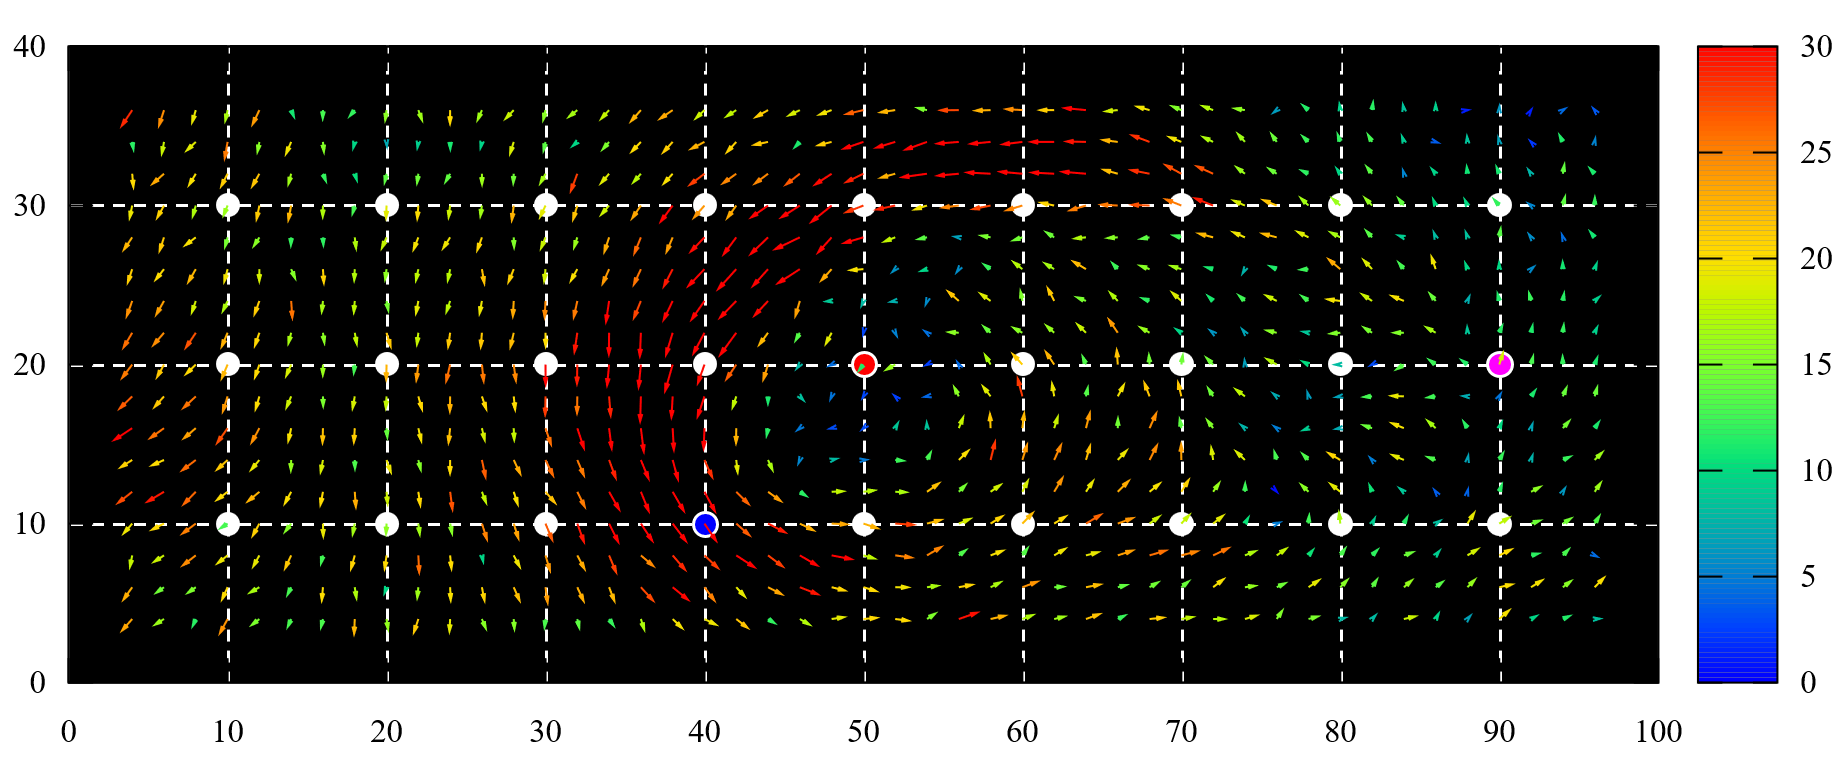
\includegraphics[width=140mm]{../images/vector_grid.png}
    \caption{Velocity vectors of delta wake : $n = 10$}
  \end{center}
  \begin{minipage}[b]{0.33\linewidth}
    \centering
    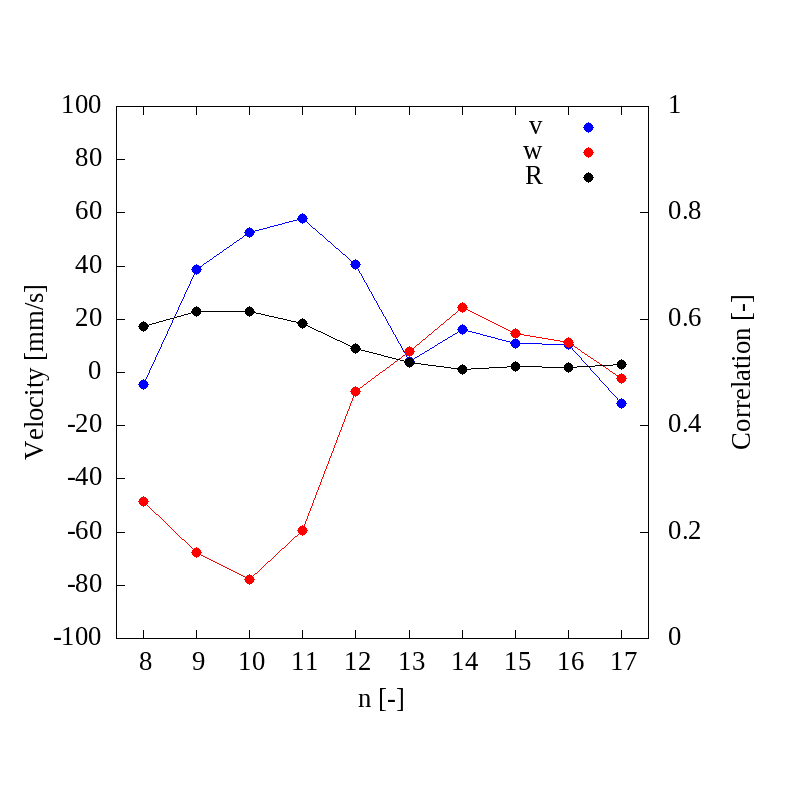
\includegraphics[keepaspectratio, scale=0.26]{../images/x=40,y=10.png}
    \subcaption{Blue : $(x,y) = (40,10)$}
  \end{minipage}
  \begin{minipage}[b]{0.33\linewidth}
    \centering
    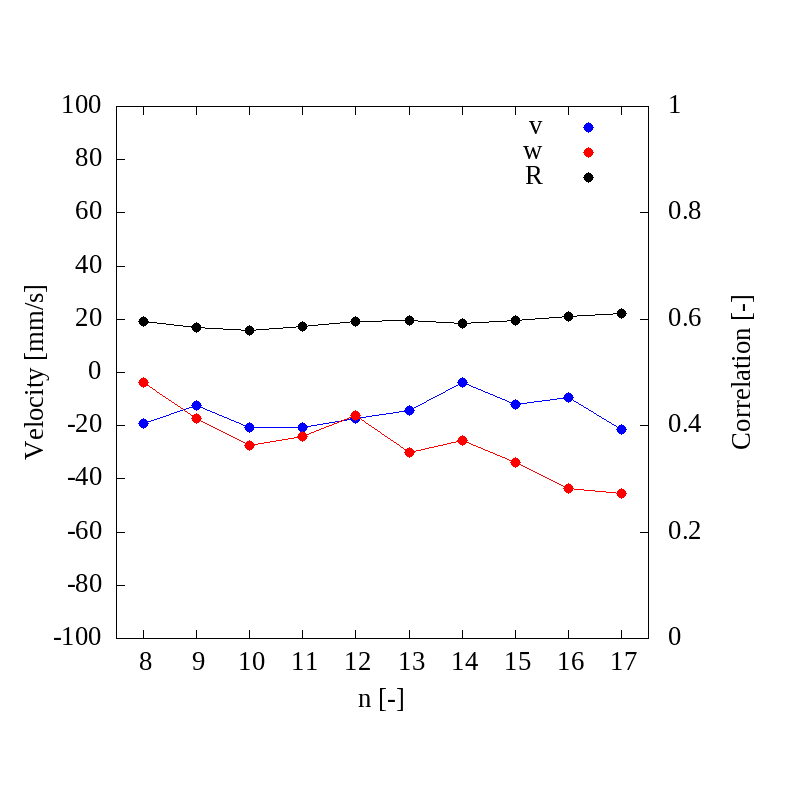
\includegraphics[keepaspectratio, scale=0.26]{../images/x=50,y=20.png}
    \subcaption{Red : $(x,y) = (50,20)$}
  \end{minipage}
  \begin{minipage}[b]{0.33\linewidth}
    \centering
    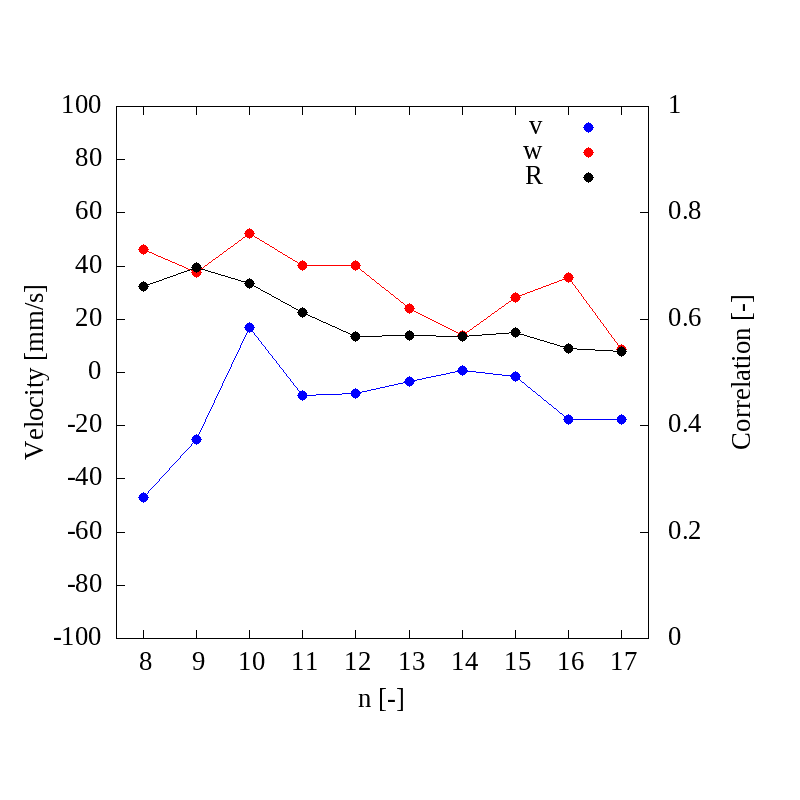
\includegraphics[keepaspectratio, scale=0.26]{../images/x=90,y=20.png}
    \subcaption{Pink : $(x,y) = (90,20)$}
  \end{minipage}
  \caption{Value transition of $v$, $w$ and $R$}
\end{figure*}

\begin{multicols*}{2}
  \section*{報告内容}
  \begin{enumerate}[1.]
    \item 枚数差の組み合わせ変更(続)
    \item 来週の予定
  \end{enumerate}
  \section{枚数差の組み合わせ変更(続)}
  枚数差の組み合わせによる各値の推移を調べた.
  撮影画像に対して Fig.1 のように $y,z$ 方向に 10 [mm] 間隔で格子点を配置し,
  その点上での $y$方向速度 $v$ [mm/s], $z$方向速度 $w$ [mm/s],および
  PTVプログラムで算出される相互相間係数 $R$ [-] の変化をFig.2に示す.
  \vskip \baselineskip
  また,Fig.2で取り上げた代表点について,青(40,10)は渦成分を大きく含むと考えられる位置,
  赤(50,20)は渦の中心付近の位置,紫(90,20)は渦の影響が少ないと考えられる位置
  を選択している.Fig.2(a) は$R$のピークが$n=10$にあることに対して,
  Fig.2(c) は$n=9$にあることがわかる,
  これより,主流方向の速度を考慮したPTVアルゴリズムの作成が必要であることがわかる.

  \section{来週の予定}
  \begin{itemize}
    \item 数値シミュレーション結果のグラフ作成
    \item ISTP-33 原稿作成
  \end{itemize}
\end{multicols*}



\end{document}